\subsection{Reproducing Dust Observations} 
In addition to comparing the observables produced by the \eda~and the forward
model with observations, we can also directly compare the dust attenuation
curves predicted by the \eda~to observations. In Figure~\ref{fig:slope}, we
present the attenuation-slope relation of \eda~dust attenuation curves for
star-forming galaxies. We use the posterior \eda~parameter values of TNG (blue)
and EAGLE (green) and present two different measurements of the UV-optical slope
used in the literature: $S = A(3000\AA)/A_V$ (left) and $\delta$, the slope
offset from the \cite{calzetti2001} curve (right). For comparison, we include
the attenuation-slope relations of GSWLC2 galaxies: \cite{salim2020} (left;
black shaded) and \cite{salim2018} (right; black hatched). We focus our
comparison to star-forming galaxies, $\log~{\rm SSFR} > -11~{yr}^{-1}$, because
attenation curves derived from observations are limited to star-forming galaxies. 

Overall, 

Observations find that star-forming galaxies with higher attenuation have
shallower slopes. 

with higher $A_V$ have
shallower slopes


At low attenuation, dust scattering dominates absoprtion so the 
attenuation curve steepens because red light scatters isotropically while blue light
scatters forward~\citep{gordon1994, witt2000, draine2003}. %, which causes more optical-to-IR light to escape the galaxy than UV light
At high attenuation dust absorption is dominant and the attenuation curve is
shallower~\citep{chevallard2013}.



We also include in Figure~\ref{fig:slope}, the attenuation-slope relations of
radiative transfer models: \cite{inoue2005} (left; dotted), \cite{chevallard2013}
(right; dot dashed), and \cite{trayford2020} (right; triangle).
For reference, we also include attenuation and slope of the Milky Way (star)
as well as the slope of the \cite{calzetti2001} curve. 








TNG and EAGLE both predict slopes within $2 < S < 5$ and centered around $S\sim
3.5$. In comparison, for the same $A_V > 0.4$ range as the DEM, observations 
find slopes within the range $2 < S < 5$~\citep{calzetti2000, burgarella2005, johnson2007,
conroy2010b, wild2011, battisti2016, battisti2017, leja2017, salim2018} in good
agreement. We also find that the DEM predicts steeper attenuation curves at 
lower attenuation. This is consistent with the established attenuation--slope
relation. 


upshot: 
The fact that our dust model reproduces all of these attenuation curve relation
is pretty remarkable. For instance, the attenuation-slope relation is a result 
of dust scattering dominating at low attenuation and dust absorption dominating 
at high attenuation. We're able to infer this relation purely from the observations 
with a model that has no priors on it. This is a good demonstration of the forward 
modeling approach and its advantages.  


%At low attenuation, dust scattering dominates absoprtion so the 
%attenuation curve steepens because red light scatters isotropically while blue light
%scatters forward~\citep{gordon1994, witt2000, draine2003}. %, which causes more optical-to-IR light to escape the galaxy than UV light
%At high attenuation dust absorption is dominant and the attenuation curve is
%shallower~\citep{chevallard2013}. For the $A_V$ range probed by the DEM, the
%$A_V$--slope relation is in good agreement with GSWLC2 galaxies~\citep[black shaded][]{salim2020}.
%They are also consistent with \cite{leja2017}. We also compare our results to
%theoretical predictions from radiative transfer models, \cite{inoue2005}
%(dotted), the radiative transfer models considered in \cite{chevallard2013}
%(dot dashed), and \cite{trayford2020} (light shaded), which all predict shallower 
%attenuation curves than observations. This is also the case for the
%\cite{narayanan2018} attenuation curves (not included). 
%\emph{The attenuation curve slopes from the DEM for are in excellent
%agreement with observations and better reproduces the observed
%attenuation--slope relation than radiative transfer models.}


\begin{figure}
\begin{center}
    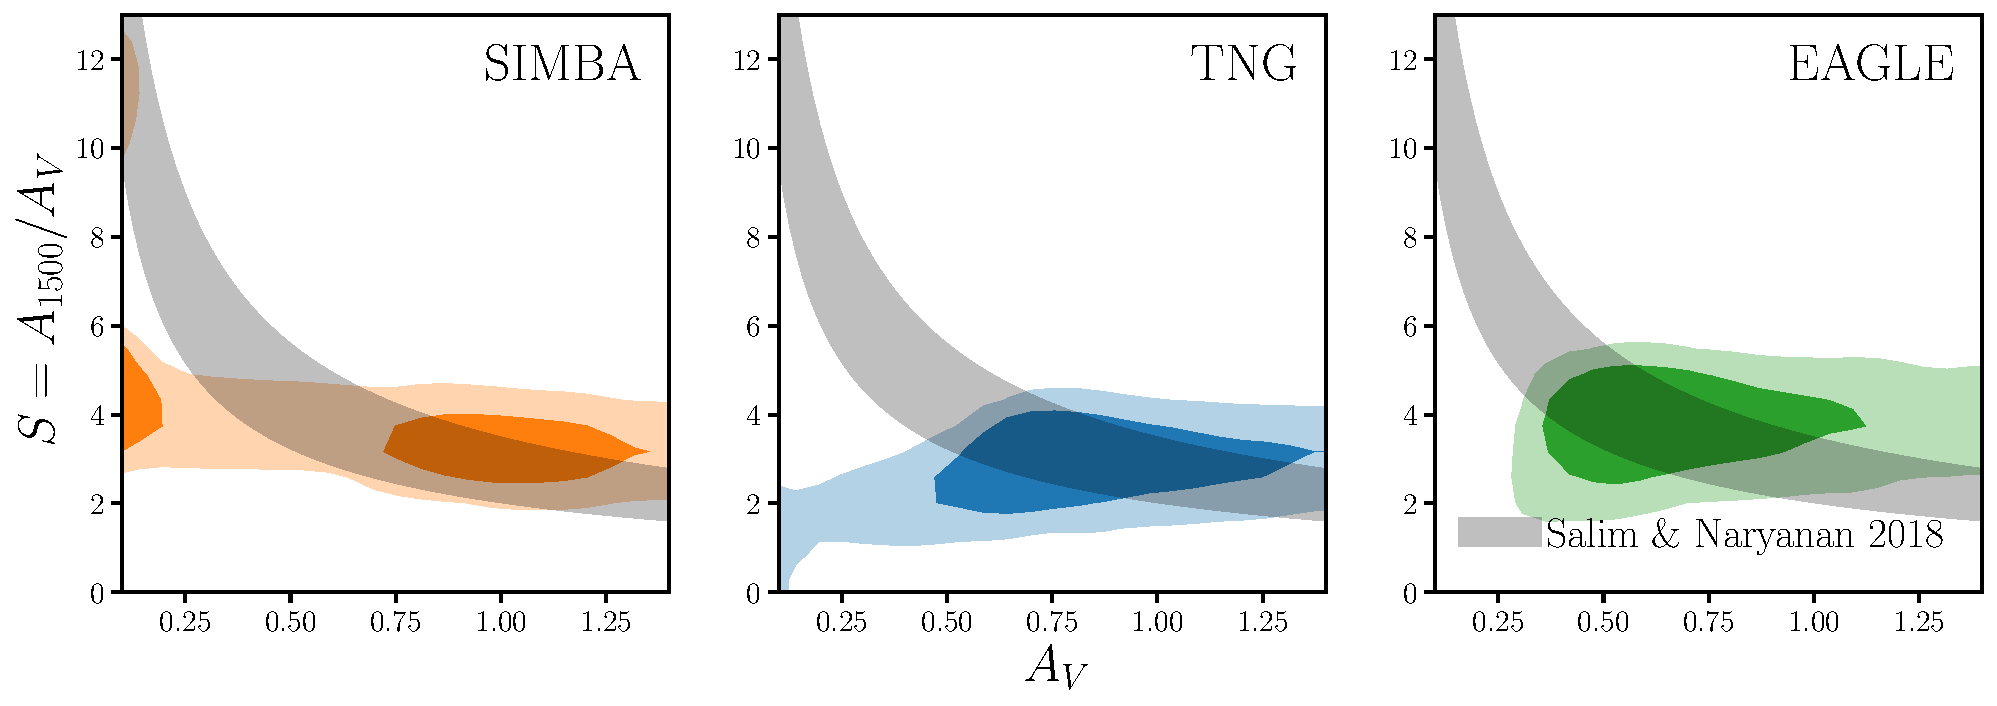
\includegraphics[width=0.85\textwidth]{figs/abc_slope_AV_all.pdf}
    \caption{\label{fig:slope}
    The attenuation-slope relation of the DEM for TNG (blue) and EAGLE (green).
    We present the relation usng two different measurements of slope, 
    commonly used in the ltierature: $S = A(1500\AA)/A_V$ (left panel) and
    the slope offset from the \cite{calzetti2001} curve, $\delta$ (right panel).
    The DEM moodels predict an attenuation-slope relation, where the slope is
    steeper at lower attenuation, consistent with both observations and
    radiative transfer models. We only include massive galaxies with $M_r <
    -20$ so galaxies in our sample have $A_V \gtrsim 0.4$. In this $A_V$ range,
    the DEM for TNG and EAGLE are in good agreement with observations~\cite{salim2020}. 
    In fact, the DEMs match the observed attenuation-slope relation better 
    than radiative transfer model that predict attenuation curves that are
    too shallow~\citep{inoue2005, chevallard2013, trayford2020}.
    }
\end{center}
\end{figure}





